\documentclass[dvipdfmx,10pt]{beamer}

\usepackage{bxdpx-beamer}% dvipdfmxなので必要
\usepackage{listings,jlisting}%ソースコード貼り付けのため
\usepackage{tikz}
\usepackage{otf}
\usetikzlibrary{positioning}
\usetikzlibrary{shadows}
\AtBeginDvi{\special{pdf:tounicode 90ms-RKSJ-UCS2}} %% しおりが文字化けしないように
\setbeamertemplate{navigation symbols}{} %% 右下のアイコンを消す

\renewcommand{\kanjifamilydefault}{\gtdefault}

\usetheme{Warsaw}
%\usetheme{Darmstadt}

\setbeamertemplate{footline}[frame number] %% スライド下のバーを消してフレーム番号を表示
\useoutertheme{shadow}                 %% 箱に影をつける
\usefonttheme{professionalfonts}       %% 数式の文字を通常の LaTeX と同じにする

\usepackage{graphicx,xcolor}%%文字の色
%\usepackage{bm}
\usepackage{ipsj}
\usepackage{color}
\usepackage{amssymb}
\usepackage{amsmath}
\usepackage{amsthm}
\usepackage{multirow,bigdelim}
\newcommand{\la}{\leftarrow}
\newcommand{\Lra}{\Longrightarrow}
\newcommand{\Lla}{\Longleftarrow}
\newcommand{\Llra}{\Longleftrightarrow}
\newcommand{\lra}{\longrightarrow}
\newcommand{\dd}{\mathop{..}}
\newcommand{\range}[2]{\{#1\dd#2\}}
\newcommand{\imp}{\Rightarrow}
\newcommand{\equ}{\Leftrightarrow}
\renewcommand{\labelenumi}{(\arabic{enumi})}
\newcommand{\alldiff}{\textrm{alldifferent}}
\newcommand{\Alldiff}{\alldiff(x_1,x_2,\ldots,x_n)}
\newcommand{\SAT}{{\tt SAT}}
\newcommand{\UNSAT}{{\tt UNSAT}}
\newcommand{\Dom}{{\it Dom}}
% \newcommand{\p}[2]{p(#1,#2)}
\newcommand{\dE}[2]{p(#1=#2)}
\newcommand{\lE}[2]{p(#1^{(#2)})}
\newcommand{\oE}[2]{p(#1\le#2)}
 % 自分用のマクロ

\title{解集合プログラミングを用いた\\ハミルトン閉路問題の解法に関する考察}
\author{平手 貴大$^1$,宋 剛秀$^2$,田村 直之$^2$,番原 睦則$^1$}
\date{日本ソフトウェア科学会第38回大会 (JSSST-2021)}
\institute{1.名古屋大学 大学院情報学研究科 \\ 2.神戸大学 情報基盤センター}
\begin{document}
%%%%%%%%%%%%%%%%%%%%%%%%%%%%%%%%%%%%%%%%%%%%%%%%%%%%%%%%%%%%%%%%%%%
\frame{\maketitle}
%%%%%%%%%%%%%%%%%%%%%%%%%%%%%%%%%%%%%%%%%%%%%%%%%%%%%%%%%%%%%%%%%%%
\begin{frame}{ハミルトン閉路問題(Hamiltonian Cycle Problem)}
  \begin{itemize}
  \item \alert{ハミルトン閉路問題}
    \begin{itemize}
    \item 与えられたグラフの全頂点をちょうど一度ずつ
      通る閉路が存在するかどうかを判定する問題.
    \item 始点と終点が一致するという閉路の条件を
      取り除けば,ハミルトン路問題となる.
    \end{itemize}
  \item \alert{最短ハミルトン閉路問題}
    \begin{itemize}
    \item グラフの辺に距離が付随しているときに,
      最短距離のハミルトン閉路を求める問題.
    \end{itemize}
  \item \alert{コスト制約付きハミルトン閉路問題}
    \begin{itemize}
    \item ハミルトン閉路問題に,距離の総和が所与の閾値以下
      (または以上)であることを制約条件として付加した問題.
    %% \item この問題に対する解の全列挙については,
    %%   現在のところ効率の良い手法は開発されていない.
    \end{itemize}
  \end{itemize}
  \begin{alertblock}{}
    本研究では,無向グラフ上のハミルトン閉路問題
    およびその関連問題を対象とする.    
  \end{alertblock}
\end{frame}
%%%%%%%%%%%%%%%%%%%%%%%%%%%%%%%%%%%%%%%%%%%%%%%%%%%%%%%%%%%%%%%%%%%
\begin{frame}{コスト制約付きハミルトン路問題[Knuth2015]}
%%%%%%%%%%%%%%%%%%%%%%%%%%%%%%%%%%%%%%%%%%%%%%%
  \begin{figure}[tb]
  \centering
  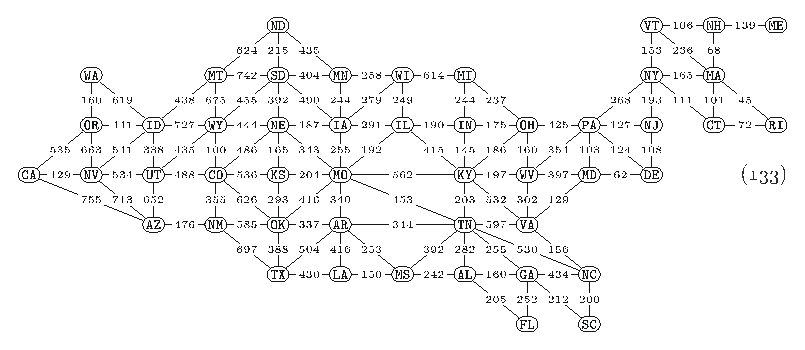
\includegraphics[width=0.8\linewidth]{fig/taocp_vol4fasc1b_p52_eq133.pdf}
  \end{figure}
%%%%%%%%%%%%%%%%%%%%%%%%%%%%%%%%%%%%%%%%%%%%%%%
  \begin{itemize}  
  \item 米国本土48州の隣接関係を表現.頂点数は48,辺の数が105
  \item 各辺に付与されている数字は,州都の間の距離(マイル).
  \end{itemize}
  \begin{block}{}
    西海岸ワシントン州 (WA) から 東海岸メーン州 (ME) までの距離の総和
    がある閾値以下であるハミルトン路を求める問題を考える.
  \end{block}
  \begin{itemize}
  \item WA から ME までのハミルトン路は 6,876,928 通り
    あり,最短ハミルトン路は 11,698 マイル.
  \item 閾値を最短距離の 10\%増 (12,868 マイル) とした場合,
    解の総数は 16,180 個.
  \end{itemize}
\end{frame}
%%%%%%%%%%%%%%%%%%%%%%%%%%%%%%%%%%%%%%%%%%%%%%%%%%%%%%%%%%%%%%%%%%%
\begin{frame}{解集合プログラミング(Answer Set Programming; ASP)}
  \begin{itemize}
  \item \alert{ASP 言語}は,一階論理に基づく知識表現言語の一種.
  \item \alert{ASP システム}は,論理プログラムから
    安定モデル意味論に基づく解集合を計算するシステム.
  \item 近年,SAT 技術を応用した高速 ASP システムが開発され,
    スケジューリング,プランニング,システム生物学,システム検証,
    制約充足問題,制約最適化問題など様々な分野への実用的応用が急速に拡大している.
  \end{itemize}

  \begin{alertblock}{ハミルトン閉路問題に ASP を用いる利点}
    \begin{itemize}
    \item ASP 言語の高い表現力を生かして,記号制約を簡潔に記述可能
    \item 組込み非閉路制約 \texttt{\#edge} 宣言を使うことにより,有向グラフの非閉路性を簡潔に記述可能.
    \item 高速な解列挙が可能.
%    \item 充足不能コアに基づく最適化
%    \item インクリメンタル ASP 解法
    \end{itemize}
  \end{alertblock}
\end{frame}
%%%%%%%%%%%%%%%%%%%%%%%%%%%%%%%%%%%%%%%%%%%%%%%%%%%%%%%%%%%%%%%%%%%
\begin{frame}{研究目的}
  \begin{alertblock}{研究目的}
  ASP 技術を活用し,大規模なハミルトン閉路問題を
    効率よく解くソルバーの実現を目指す.
  \end{alertblock}
  \begin{block}{研究内容}
    \begin{enumerate}
    \item \structure{ハミルトン閉路問題を解く3種類の ASP 符号化を考案.}
      \begin{itemize}
      \item \textsf{undirected}符号化, \textsf{directed}符号化, \textsf{acyclicity}符号化.
      \item ASP の \alert{ルール 10 個程度で簡潔に表現}できることを確認.
      \end{itemize}
    \item \structure{最短ハミルトン閉路,コスト制約付きハミルトン閉路への拡張}
    \item \structure{既存のベンチマーク問題集を用いた評価実験.}
      \begin{itemize}
        \item \alert{FHCP Challenge 国際競技会}で使用された頂点数が
          66個から9,528個のハミルトン閉路問題のインスタンス(全1001問)
          を使用した.
        \item directed 符号化が 879 問と最も多くの問題を解き,他の符号
          化と比較して,その優位性が確認できた.
        \item FHCP Challenge 競技会の優勝ソルバーは985問,2位は614問で
          あることから,directed 符号化は\alert{実質2位}の成績に相当する.
        \end{itemize}
    \end{enumerate}
  \end{block}
\end{frame}
%%%%%%%%%%%%%%%%%%%%%%%%%%%%%%%%%%%%%%%%%%%%%%%%%%%%%%%%%%%%%%%%%%%
\begin{frame}{ASP 言語の構文}
\begin{alertblock}{}\centering
  ASPの言語は論理プログラムをベースとする\footnotemark.
\end{alertblock}

\begin{itemize}
  \item \structure{論理プログラム}とは,
	以下の形式の\structure{ルール}
	の有限集合である.
\begin{block}{}
    \[
	\underbrace{a_0}_{\textrm{ヘッド}}\ \texttt{:-}\
	\underbrace{a_1\texttt{,}\dots\texttt{,}a_m\texttt{,}
	\texttt{not}\ {a_{m+1}}\texttt{,}\dots\texttt{,}
	\texttt{not}\ {a_n}\texttt{.}}_{\textrm{ボディ}}
    \]
\end{block}
    $0\leq m\leq n$ であり,
    各$a_i$はアトム,
    \texttt{not}は\structure{デフォルトの否定},
    ``\texttt{,}''は連言を表す.
    \pause
  \item \alert{\bf 直観的な意味}は「$a_1,\ldots,a_m$がすべて成り立ち,
    $a_{m+1},\ldots,a_n$のそれぞれが成り立たないならば,$a_0$が成り立つ」である.
    \pause
  \item ボディが空のルールは\structure{ファクト}と呼ばれ,
	``\texttt{:-}''は省略できる.
  \item ヘッドが空のルールは\structure{一貫性制約}と呼ばれる.
	``\(\texttt{:-}\ \texttt{not}\ a_1\texttt{,} {a_{2}}\texttt{.}\)''は,
	「$a_2$が成り立つならば,$a_1$が成り立つ」となる.
\end{itemize}
 \footnotetext{本発表では標準論理プログラムを単に論理プログラムと呼ぶ.}
\end{frame}
%%%%%%%%%%%%%%%%%%%%%%%%%%%%%%%%%%%%%%%%%%%%%%%%%%%%%%%%%%%%%%%%%%%
\begin{frame}{拡張構文}
\begin{alertblock}{}\centering
 ASP言語には,組合せ問題やグラフ問題を解く際に便利な構文が用意されて
 いる.
\end{alertblock}

\begin{itemize}
\item \structure{選択子}\\
  \begin{center}
   \code{\{}\(a_1\texttt{;}\dots\texttt{;}a_n\)\code{\}}\\
  \end{center}
  アトム集合\(\{a_1,\dots,a_n\}\)の任意の部分集合が成り立つことを意味
  する.
\item \structure{個数制約}
  \begin{center}
   $lb$\ \code{\{}\(a_1\texttt{;}\dots\texttt{;}a_n\)\code{\}}\ $ub$
  \end{center}
  $a_1,\dots,a_n$のうち,$lb$個以上$ub$個以下が成り立つことを意味する.
\item \structure{\texttt{\#edge}宣言}
  \[
      \texttt{\#edge(X,Y): 
      arc(X,Y)}.
  \]
  \code{arc(X,Y)}を満たす有向辺\code{X}~$\rightarrow$~\code{Y}
  を辺集合としてもつグラフが,閉路をもたないことを保証する.
\end{itemize}
\vfill
\pause
組合せ最適化問題を解くために,最小化関数 (\structure{\texttt{\#minimize}}) 
と最大化関数 (\structure{\texttt{\#maximize}}) 等も用意されている.
\end{frame}
%%%%%%%%%%%%%%%%%%%%%%%%%%%%%%%%%%%%%%%%%%%%%%%%%%%%%%%%%%%%%%%%%%%
\begin{frame}[noframenumbering]{ASP を用いたハミルトン閉路問題(HCP)の解法}
%%%%%%%%
\begin{figure}[h]
  \centering
  \thicklines
  \setlength{\unitlength}{1.0pt}
  \small\footnotesize\scriptsize
  \begin{picture}(280,57)(4,-10)
    \put(  0, 20){\dashbox(50,24){\shortstack{HCP\\インスタンス}}}
    \put( 60, 20){\framebox(50,24){変換器}}
    \put(120, 20){\alert{\dashbox(50,24){\shortstack{ASPファクト}}}}
    \put(120,-10){\alert{\dashbox(50,24){\shortstack{ASP符号化\\\tiny{(論理プログラム)}}}}}
    \put(180, 20){\framebox(50,24){ASPシステム}}
    \put(240, 20){\dashbox(50,24){HCPの解}}
    \put( 50, 32){\vector(1,0){10}}
    \put(110, 32){\vector(1,0){10}}
    \put(170, 32){\vector(1,0){10}}
    \put(230, 32){\vector(1,0){10}}
    \put(170, +2){\line(1,0){4}}
    \put(174, +2){\line(0,1){30}}
  \end{picture}  
%\caption{ASP を用いたハミルトン閉路問題(HCP)の解法}
\label{fig:arch}
\end{figure}
%%%%

\begin{itemize}
\item 与えられたHCPインスタンスを ASP ファクトに変換する.
\item ASP ファクトをハミルトン閉路問題を解く論理プログラム(ASP符号化)と結合し,
      ASP システムに入力する.
\item ASP システムによって解が計算される.
\end{itemize}
\end{frame}
%%%%%%%%%%%%%%%%%%%%%%%%%%%%%%%%%%%%%%%%%%%%%%%%%%%%%%%%%%%%%%%%%%%
\begin{frame}{ハミルトン閉路問題の ASP ファクト表現}
%%%%%%%%%%%%%%%%%%%%%%%%%%%%%%
\begin{center}
\scalebox{0.9}[0.9]{\begin{tikzpicture}
  %ノード1  
  \draw(4,2) circle (0.5)
  node[at={(4.1,2.1)}] {
    \begin{tabular}{c}
      1
    \end{tabular}
  };
  %ノード2  
  \draw(4,0) circle (0.5)
  node[at={(4.1,0.1)}] {
    \begin{tabular}{c}
      2
    \end{tabular}
  };
  %ノード3  
  \draw(6,2) circle (0.5)
  node[at={(6.1,2.1)}] {
    \begin{tabular}{c}
      3
    \end{tabular}
  };
  %ノード4  
  \draw(6,0) circle (0.5)
  node[at={(6.1,0.1)}] {
    \begin{tabular}{c}
      4
    \end{tabular}
  };
  %ノード5  
  \draw(8,2) circle (0.5)
  node[at={(8.1,2.1)}] {
    \begin{tabular}{c}
      5
    \end{tabular}
  };
  %ノード6  
  \draw(8,0) circle (0.5)
  node[at={(8.1,0.1)}] {
    \begin{tabular}{c}
      6
    \end{tabular}
  };
\draw(4,0.5) --(4,1.5);
\draw(6,0.5) --(6,1.5);
\draw(8,0.5) --(8,1.5);
\draw(4.5,0) --(5.5,0);
\draw(4.5,2) --(5.5,2);
\draw(6.5,0) --(7.5,0);
\draw(6.5,2) --(7.5,2);
\end{tikzpicture}
}
\end{center}
%%%%%%%%%%%%%%%%%%%%%%%%%%%%%%

%%%%%%%%%%%%%%%%%%%%%%%%%%%%%%
\begin{exampleblock}{}
\lstinputlisting[frame=none,numbers=none]{code/graph_example.lp} 
\end{exampleblock}
%%%%%%%%%%%%%%%%%%%%%%%%%%%%%%
\end{frame}
%%%%%%%%%%%%%%%%%%%%%%%%%%%%%%%%%%%%%%%%%%%%%%%%%%%%%%%%%%%%%%%%%%%
\begin{frame}{考案したハミルトン閉路問題の ASP 符号化}
  \begin{block}{ハミルトン閉路問題の制約}
    与えられた無向グラフ$G= (V,E)$上に,以下の2つの制約を満たす
    部分グラフ$G'= (V,E')$が存在するか判定する問題.
    \begin{itemize}
    \item $G'$の各頂点の次数が2.(\alert{次数制約})
    \item $G'$が連結.(\alert{連結制約})
    \end{itemize}
  \end{block}
  \begin{itemize}
  \item \alert{\textsf{undirected}符号化}
    \begin{itemize}
    \item ハミルトン閉路問題の次数制約と連結制約を簡潔に表現した符号化.
    \end{itemize}
  \item \alert{\textsf{directed}符号化}
    \begin{itemize}
    \item \textsf{undirected}符号化をベースに,与えられた無向グラフを
      有向グラフ化して解く符号化.
    \end{itemize}
  \item \alert{\textsf{acyclicity}符号化}
    \begin{itemize}
    \item \textsf{directed}符号化をベースに,連結制約に代わり
      部分閉路を禁止する制約を使用.
      \item \texttt{\#edge} を用いて,部分閉路を禁止する制約を簡潔に表現.
    \end{itemize}
  \end{itemize}
\end{frame}
%%%%%%%%%%%%%%%%%%%%%%%%%%%%%%%%%%%%%%%%%%%%%%%%%%%%%%%%%%%%%%%%%%%
\begin{frame}{\textsf{undirected}符号化}
\begin{exampleblock}{}
%%%%%%%%%%%%%%%%%%%%%%%%%%%%%%
\lstinputlisting[numbers=none, frame=none]{code/hc1.lp}
%%%%%%%%%%%%%%%%%%%%%%%%%%%%%% 
\end{exampleblock}
\begin{itemize}
\item \code{(1)}は,各辺\code{edge(X,Y)}に対して,その辺がハミルト
      ン閉路に含まれるかどうかを意味するアトム\code{in(X,Y)}を導入する.
\item 次数制約は\code{(2)}で表される.
      各頂点\code{node(X)}に対し,その次数が2に等しくなることを
      表す.
\item 連結制約は\code{(3)--(6)}行目のルールで表される.
      \code{(3)--(5)}は,ある頂点\code{X}が始点\code{s}から到達可能であることを意味する補助ア
      トム\code{reached(X)}を導入する.
      \code{(6)}は,すべての頂点が始点から到達可能でなければならないこ
      とを表す.
\end{itemize}
\end{frame}
%%%%%%%%%%%%%%%%%%%%%%%%%%%%%%%%%%%%%%%%%%%%%%%%%%%%%%%%%%%%%%%%%%%
\begin{frame}{ASP システムの出力}
%%%%%%%%%%%%%%%%%%%%%%%%%%%%%%
\begin{figure}[t]
\begin{center}
\begin{tikzpicture}
  %ノード1  
  \draw(4,2) circle (0.5)
  node[at={(4.0,2.0)}] {
    \begin{tabular}{c}
      1
    \end{tabular}
  };
  %ノード2  
  \draw(4,0) circle (0.5)
  node[at={(4.0,0.0)}] {
    \begin{tabular}{c}
      2
    \end{tabular}
  };
  %ノード3  
  \draw(6,2) circle (0.5)
  node[at={(6.0,2.0)}] {
    \begin{tabular}{c}
      3
    \end{tabular}
  };
  %ノード4  
  \draw(6,0) circle (0.5)
  node[at={(6.0,0.0)}] {
    \begin{tabular}{c}
      4
    \end{tabular}
  };
  %ノード5  
  \draw(8,2) circle (0.5)
  node[at={(8.0,2.0)}] {
    \begin{tabular}{c}
      5
    \end{tabular}
  };
  %ノード6  
  \draw(8,0) circle (0.5)
  node[at={(8.0,0.0)}] {
    \begin{tabular}{c}
      6
    \end{tabular}
  };
  \draw[red, line width=2pt](4,0.5) --(4,1.5)
  node[at={(3.8,1.0)}] {};
  \draw(6,0.5) --(6,1.5)
  node[at={(5.8,1.0)}] {};
  \draw[red, line width=2pt](8,0.5) --(8,1.5)
  node[at={(7.8,1.0)}] {};
  \draw[red, line width=2pt](4.5,0) --(5.5,0)
  node[at={(5.0,0.4)}] {};
  \draw[red, line width=2pt](4.5,2) --(5.5,2)
  node[at={(5.0,2.4)}] {};
  \draw[red, line width=2pt](6.5,0) --(7.5,0)
  node[at={(7.0,0.4)}] {};
  \draw[red, line width=2pt](6.5,2) --(7.5,2)
  node[at={(7.0,2.4)}] {};
\end{tikzpicture}

\end{center}
\end{figure}
%%%%%%%%%%%%%%%%%%%%%%%%%%%%%%
\begin{exampleblock}{}
\lstinputlisting[numbers=none, frame=none]{code/output.txt}
\end{exampleblock}
%%%%%%%%%%%%%%%%%%%%%%%%%%%%%%
\end{frame}
%%%%%%%%%%%%%%%%%%%%%%%%%%%%%%%%%%%%%%%%%%%%%%%%%%%%%%%%%%%%%%%%%%%
\begin{frame}{\textsf{directed}符号化}
\begin{exampleblock}{}
%%%%%%%%%%%%%%%%%%%%%%%%%%%%%%
\lstinputlisting[numbers=none, frame=none]{code/hc2.lp}
%%%%%%%%%%%%%%%%%%%%%%%%%%%%%%
\end{exampleblock}
\begin{itemize}
\item \code{(1)}は,無向グラフの有向グラフ化を行う.
      与えられた無向グラフの各辺\code{edge(X,Y)}に対して,
      \code{in(X,Y)}と\code{in(Y,X)}を導入し,
      二つの弧\code{X}$\rightarrow$\code{Y}と\code{Y}$\rightarrow$\code{X}のうち
      高々1個がハミルトン閉路に含まれることを表す.
\item \code{(7)}は,対称解を除去する制約である.
      有向グラフ化した場合,無向グラフ上の各ハミルトン閉路に対して,
      右回りと左回りの2つの対称なハミルトン閉路が存在する.
\end{itemize}
\end{frame}
%%%%%%%%%%%%%%%%%%%%%%%%%%%%%%%%%%%%%%%%%%%%%%%%%%%%%%%%%%%%%%%%%%%
\begin{frame}{\textsf{directed}符号化(続き)}
\begin{exampleblock}{}
%%%%%%%%%%%%%%%%%%%%%%%%%%%%%%
\lstinputlisting[numbers=none, frame=none]{code/hc2.lp}
%%%%%%%%%%%%%%%%%%%%%%%%%%%%%%
\end{exampleblock}
\begin{itemize}
\item 次数制約は\code{(2)--(3)}行目のルールで表される.
      \code{(2)}は,各頂点\code{node(X)}の出次数が1に等しいことを表す.
      \code{(3)}は入次数が1に等しいことを表す.
\item 連結制約は,\textsf{directed}符号化と同様に,
      補助アトム\code{reached/1}を使って表される(\code{(4)--(6)}).
\end{itemize}
\end{frame}
%%%%%%%%%%%%%%%%%%%%%%%%%%%%%%%%%%%%%%%%%%%%%%%%%%%%%%%%%%%%%%%%%%%
\begin{frame}{\textsf{acyclicity}符号化}
\begin{exampleblock}{}
%%%%%%%%%%%%%%%%%%%%%%%%%%%%%%
\lstinputlisting[numbers=none, frame=none]{code/hc3.lp}
%%%%%%%%%%%%%%%%%%%%%%%%%%%%%% 
\end{exampleblock}
\begin{itemize}
\item \textsf{directed}符号化をベースに,
      連結制約を部分閉路を禁止する制約に置き換えたものである.
\item \code{(4)}は,始点\code{s}を含まない弧\code{in(X,Y)}
      の集合をもつ有向グラフが閉路を含まないことを,
      \textit{clingo}の\code{\#edge}宣言を使って簡潔に表している.
\end{itemize}
\end{frame}
%%%%%%%%%%%%%%%%%%%%%%%%%%%%%%%%%%%%%%%%%%%%%%%%%%%%%%%%%%%%%%%%%%%
\begin{frame}[noframenumbering]{符号化の拡張}
\begin{itemize}
%%%%%%%%%%%%%%%%%%%%%%%%%%%%%%
\begin{exampleblock}{}
\lstinputlisting[frame=none, numbers=none]{code/obj_minimize.lp} 
\end{exampleblock}
%%%%%%%%%%%%%%%%%%%%%%%%%%%%%%    
  \item \alert{最短ハミルトン閉路問題}の ASP 符号化では,
	目的関数を追加する.
  \item このルールは,ハミルトン閉路に含まれる
	各辺 \code{X} – \code{Y} の距離 \code{C} 
	の総和を最小化する.
%%%%%%%%%%%%%%%%%%%%%%%%%%%%%%
\begin{exampleblock}{}
\lstinputlisting[frame=none, numbers=none]{code/cost_constraint.lp}
\end{exampleblock}
%%%%%%%%%%%%%%%%%%%%%%%%%%%%%%    
  \item \alert{コスト制約付きハミルトン閉路問題}の ASP 符号化では,
	コスト制約を追加する.
  \item このルールは,ハミルトン閉路上の辺の距離の総和が
	閾値 \code{c} 以下であることを表す.
%%%%%%%%%%%%%%%%%%%%%%%%%%%%%%
\begin{exampleblock}{}
\lstinputlisting[frame=none, numbers=none]{code/cost_both.lp}
\end{exampleblock}
%%%%%%%%%%%%%%%%%%%%%%%%%%%%%%    
  \item \textsf{directed}と\textsf{acyclicity}について,
	距離を有向グラフ化に対応させる.
  \item 各辺\code{X}–\code{Y}の距離 \code{C} を弧\code{X} $\rightarrow$ \code{Y},
	\code{Y} $\rightarrow$ \code{X}に付与する.
\end{itemize}
\end{frame}
%%%%%%%%%%%%%%%%%%%%%%%%%%%%%%%%%%%%%%%%%%%%%%%%%%%%%%%%%%%%%%%%%%%
\begin{frame}{実験概要}
  考案した ASP 符号化の性能を評価するために実験を行った.
  \begin{itemize}
  \item \structure{比較する ASP 符号化}:
    \begin{itemize}
    \item \textsf{undirected}符号化
    \item \textsf{directed}符号化
    \item \textsf{acyclicity}符号化
    \end{itemize}
  \item \structure{対象とする問題}:
    \begin{enumerate}
    \item ハミルトン閉路問題: 計1001問
      \begin{itemize}
      \item \structure{制限時間}: 30分/問
      %% \item \structure{オプション}: \textit{trendy}
      %% \item \structure{ベンチマーク問題}:\\
        %% \textsf{color04},
        %% \textsf{complete},
        %% \textsf{knight},
        %% \textsf{tsplib},
        %% \textsf{grid},
        %% \textsf{random}
      \end{itemize}
    \item 最短ハミルトン路問題: 計7問
      \begin{itemize}
      \item \structure{制限時間}: 3時間/問
      %% \item \structure{オプション}: \textit{trendy}
      %% \item \structure{ベンチマーク問題}: \textsf{usmap}, \textsf{grid}
      \end{itemize}
    \item コスト制約付きハミルトン路問題(解の全列挙): 計10問
      \begin{itemize}
      \item \structure{制限時間}: 3時間/問
      %% \item \structure{オプション}: \textit{crafty}
      %% \item \structure{ベンチマーク問題}: \textsf{usmap} (閾値: 10問)
      \end{itemize}
    \end{enumerate}
  \item \structure{ASP システム}: \textit{clingo-5.5.0}
  \item \structure{実験環境}: Mac mini Intel Corei7 3.2GHz, 64GBメモリ
  \end{itemize}
\end{frame}
%%%%%%%%%%%%%%%%%%%%%%%%%%%%%%%%%%%%%%%%%%%%%%%%%%%%%%%%%%%%%%%%%%%
\begin{frame}{ハミルトン閉路問題のベンチマーク問題}
\begin{block}{使用したベンチマーク問題の説明}
Flinders Hamiltonian Cycle Project(FHCP)\footnotemark で
公開されている HCP インスタンス集合である.
\begin{itemize}
 \item ハミルトン閉路が存在する\alert{ SAT インスタンス(全1,001問)}である.
 \item 頂点数は66個から9,528個で,平均で3000以上のサイズである.
 \item \textit{Concorde},\textit{LKH},\textit{SLH} の
       2つ以上で,解くことが難しいと判断されており,
       標準的なHCPヒューリスティックスでは解くのが難しいように設計されている.
\end{itemize}
\end{block}
\footnotetext{https://sites.flinders.edu.au/flinders-hamiltonian-cycle-project/}
\end{frame}
%%%%%%%%%%%%%%%%%%%%%%%%%%%%%%%%%%%%%%%%%%%%%%%%%%%%%%%%%%%%%%%%%%%
\begin{frame}{ハミルトン閉路問題の実験結果(解けた問題数)}
%%%%%%%%%%%%%%%%%%%%%%%%%%%%%%%%%%%%%%%%%%%%%%%
\begin{table*}[t]\footnotesize
  \centering
% \tabcolsep = 0.8mm
% \renewcommand{\arraystretch}{1.2}
  \begin{tabular}{lr||r|r|r}
    頂点数 & 問題数 & \textsf{undirected} & \textsf{directed} & \textsf{acyclicity}\\
   \hline
    $\:\:\:\:\:\,\, 0 \leq |V| < 1000$  & 171   & 156   & \textbf{171}   & 155  \\
    $1000 \leq |V| < 2000$  & 165   & 120   & \textbf{158}   & 124  \\
    $2000 \leq |V| < 3000$  & 177   & 125   & \textbf{162}   & 73   \\
    $3000 \leq |V| < 4000$  & 185   & 104   & \textbf{148}   & 42   \\
    $4000 \leq |V| < 5000$  & 128   & 92    & \textbf{104}   & 28   \\
    $5000 \leq |V| < 6000$  & 80    & 63    & \textbf{68}    & 23   \\
    $6000 \leq |V| < 7000$  & 55    & 39    & \textbf{43}    & 21   \\
    $7000 \leq |V| < 8000$  & 28    & 12    & \textbf{14}    & 5    \\
    $8000 \leq |V| < 9000$  & 10    & 2     & \textbf{5}     & 1    \\
    $9000 \leq |V| < 10000$ & 2     & \textbf{2}     & \textbf{2}     & 1    \\
   \hline
    合計 & 1001 & 715   & \textbf{875}   & 473  
  \end{tabular}
  \vskip .5em
  \caption{ハミルトン閉路問題: 解けた問題数}
  \label{sat_table}
\end{table*}
%label{sat_table}
%%%%%%%%%%%%%%%%%%%%%%%%%%%%%%%%%%%%%%%%%%%%%%%
\begin{itemize}
\item 1列目はHCPインスタンスの頂点数の範囲,2列目は問題数,
      3列目以降は各符号化で解けた問題数を示している.
\item \textsf{directed}符号化が879問を解き,もっとも多くの問題を解いた.
\item \textsf{directed}符号化は,どの頂点数の範囲においても
      他の符号化と同じかより多くの問題を解いており,その優位性が確認できる.
\end{itemize}
\end{frame}
%%%%%%%%%%%%%%%%%%%%%%%%%%%%%%%%%%%%%%%%%%%%%%%%%%%%%%%%%%%%%%%%%%%
\begin{frame}{ハミルトン閉路問題の実験結果(カクタスプロット)}
%%%%%%%%%%%%%%%%%%%%%%%%%%%%%%%%%%%%%%%%%%%%%%%
\begin{figure}[tb]
\begin{center}
  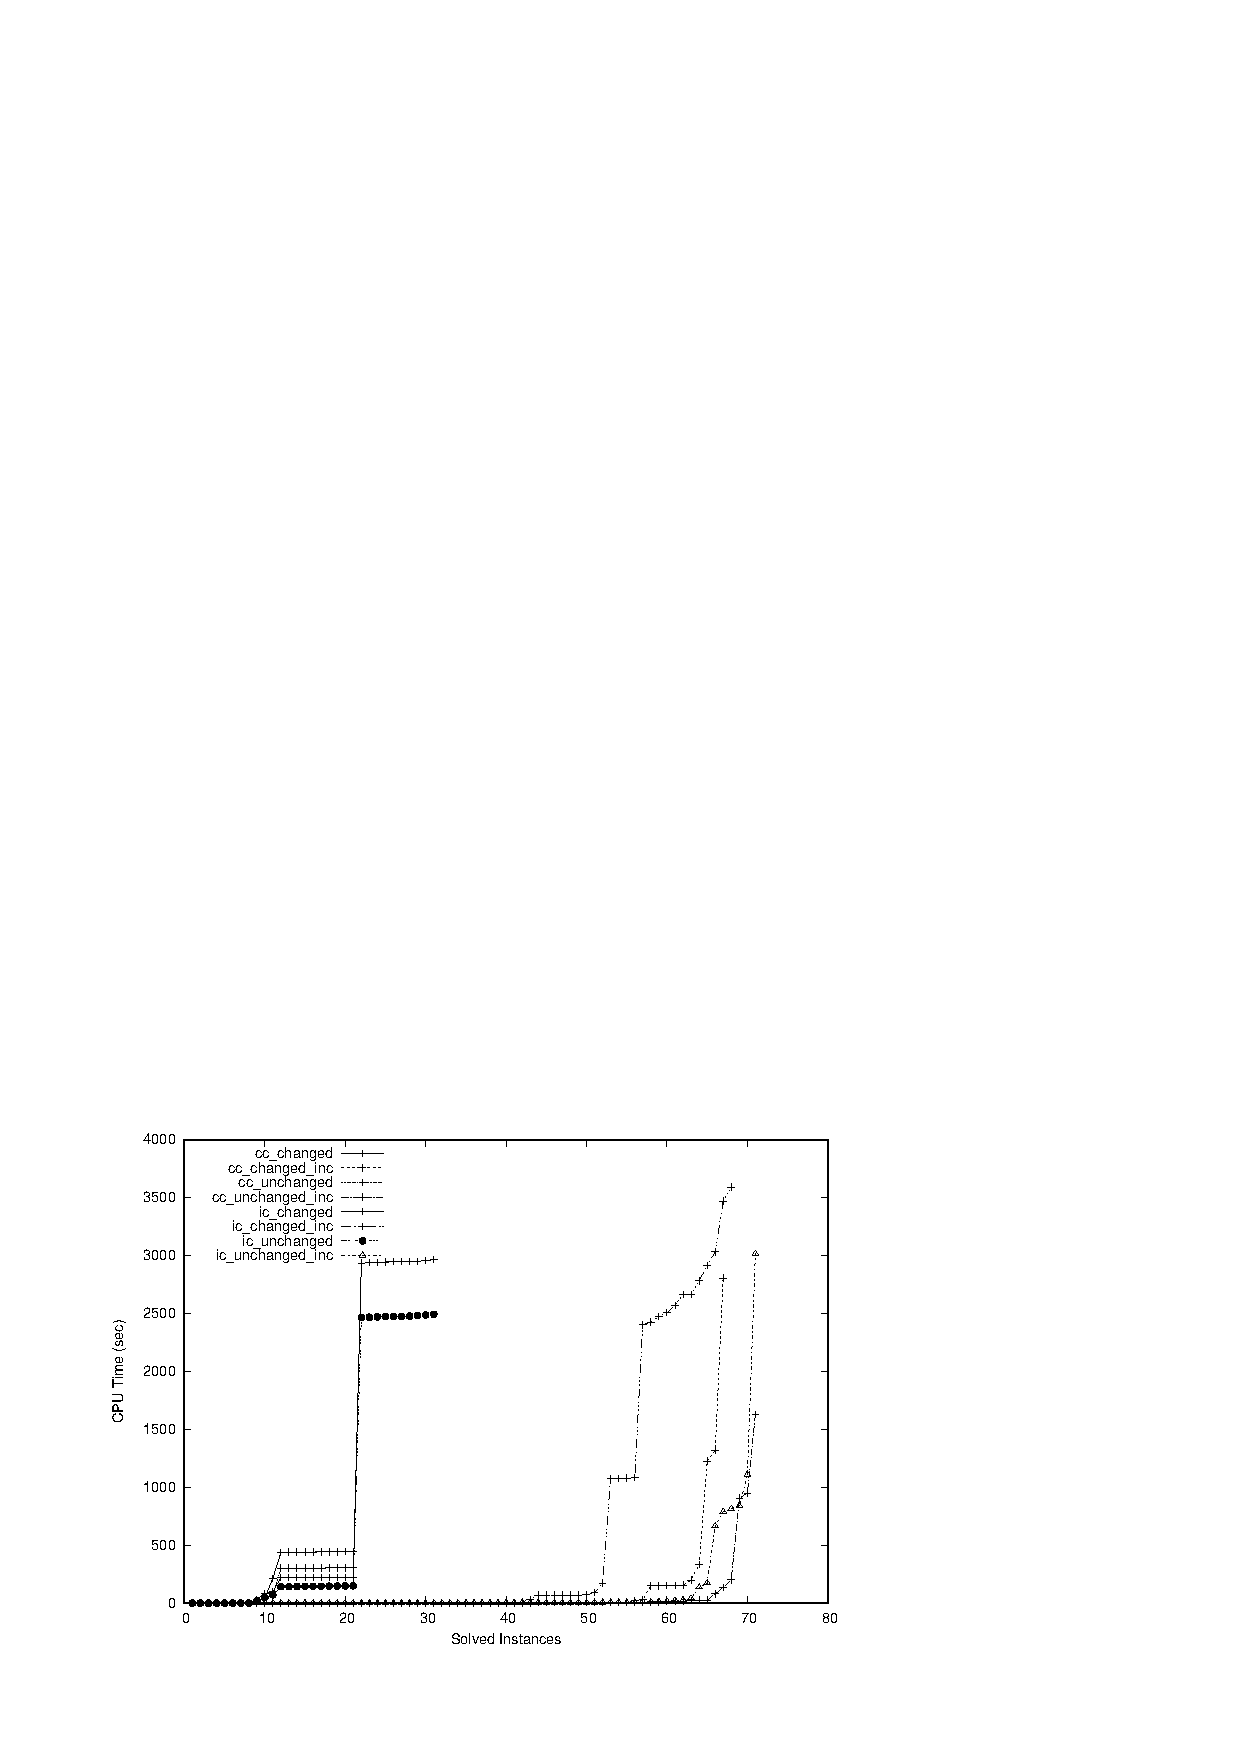
\includegraphics[width=0.7\linewidth]{fig/cactus.png}
%\caption{ハミルトン閉路問題: カクタスプロット (\textsf{SAT+UNSAT})}
\label{cactus}
\end{center}
\end{figure}
%%%%%%%%%%%%%%%%%%%%%%%%%%%%%%%%%%%%%%%%%%%%%%%
\begin{itemize}
\item \textsf{directed}符号化が,他の2つの符号化と比較して,
      より多くの問題を高速に解いていることが確認できる.
\end{itemize}
\end{frame}
%%%%%%%%%%%%%%%%%%%%%%%%%%%%%%%%%%%%%%%%%%%%%%%%%%%%%%%%%%%%%%%%%%%
\begin{frame}{実験結果の考察}
%%%%%%%%%%%%%%%%%%%%%%%%%%%%%%
\begin{center}
% \scalebox{0.9}[0.9]{\begin{tikzpicture}
% 座標設定
\coordinate (O) at (0,0);
\coordinate (NE) at (5,4.5);
\coordinate (SW) at (-5,-3.5);
% 円の描画
\filldraw[draw=black, fill=white,line width=1pt] (SW) rectangle (NE);
\filldraw[draw=\venncolorA,fill=\venncolorA,fill opacity=0.1,line width=1pt] \venncircleA;
\filldraw[draw=\venncolorB,fill=\venncolorB,fill opacity=0.1,line width=1pt] \venncircleB;
\filldraw[draw=\venncolorC,fill=\venncolorC,fill opacity=0.1,line width=1pt] \venncircleC;
% ラベルの描画
  \node[set label] at (O |- NE) {$U$ (計1001問)};
  \node[set label,text=\venncolorA] at (90:\vennradius+0.85*\vennradius) {undirected};
  \node[set label,text=\venncolorB] at (-150:\vennradius+\vennratio*\vennradius) {acyclicity};
  \node[set label,text=\venncolorC] at (-30:\vennradius+\vennratio*\vennradius) {directed};
  \node[font=\Large] at (90:\vennradius) {23};
  \node[font=\Large] at (-150:\vennradius) {0};
  \node[font=\Large] at (-30:\vennradius) {107};
  \node[font=\Large] at (30:1.1)  {291};
  \node[font=\Large] at (150:1.1) {1};
  \node[font=\Large] at (-90:1.1) {81};
  \node[font=\Large] at (0:0)   {400};
  \node[font=\Large] at (155:4) {98};
\end{tikzpicture}
}
\includegraphics[width=0.5\linewidth]{fig/venn.jpeg}
\end{center}
%%%%%%%%%%%%%%%%%%%%%%%%%%%%%%
\begin{itemize}
 \item \texttt{directed}は,\texttt{acyclicity}が解いた482問について,
       1問を除いて全て解いている.
 \item \texttt{directed}が解けなかった問題の中で,
       \texttt{undirected}が解いたものが24問存在する.
 \item いずれかの符号化で解ける問題の数は,903問である.
\end{itemize}
\end{frame}
%%%%%%%%%%%%%%%%%%%%%%%%%%%%%%%%%%%%%%%%%%%%%%%%%%%%%%%%%%%%%%%%%%%
\begin{frame}{他のアプローチとの比較}
本実験で使用したハミルトン閉路問題の問題集は,
2015年から2016年にかけて行われた FHCP Challenge 競技会
で使用されたものである.
\begin{itemize}
\item 1位 985 問(整数計画ソルバー CPLEX)
\item 2位 614 問(SATソルバー)
\item 3--5位 488,464,385問
\end{itemize}
\begin{alertblock}{}
879問を解いた\textsf{directed}符号化は,ASP 
のルール10個程度の簡潔なプログラムであるにもか
かわらず,実質2位の成績に相当する.
\end{alertblock}
\end{frame}
%%%%%%%%%%%%%%%%%%%%%%%%%%%%%%%%%%%%%%%%%%%%%%%%%%%%%%%%%%%%%%%%%%%
\begin{frame}{最短ハミルトン路問題の実験結果(最良値)}
 %%%%%%%%%%%%%%%%%%%%%%%%%%%%%%
\begin{table}[t]\footnotesize
  \caption{最短ハミルトン閉路問題: 得られた目的関数の値}
  \label{min_table_tr}
  \tabcolsep = 2mm
  %\renewcommand{\arraystretch}{1.0}
  \vskip .5em
  \centering
  \begin{tabular}{l|rrr}\hline
     問題 & \textsf{undirected} & \textsf{directed} & \textsf{acyclicity} \\
    \hline
    grid5&50,656*&50,656*&50,656* \\
    grid6&68,656*&68,656*&68,656* \\
    grid7&91,822*&91,822*&91,822* \\
    grid8&113,250&\textcolor{red}{112,916}&113,277 \\
    grid9&\textcolor{red}{142,502}&143,326&143,660 \\
    grid10&\textcolor{red}{172,703}&174,866&175,999 \\
    grid11&\textcolor{red}{200,399}&204,456&200,638 \\
    grid12&\textcolor{red}{231,278}&239,275&232,012 \\
    grid13&\textcolor{red}{276,692}&276,926&276,899 \\
    grid14&317,617&\textcolor{red}{317,144}&317,676 \\
    grid15&\textcolor{red}{375,906}&376,809&376,210 \\
    grid16&421,249&\textcolor{red}{419,737}&423,753 \\
    US48&11,698*&11,698*&11,698* \\
    \hline
    最適値と最良値の数 & 10 & 7 & 4\\    \hline
  \end{tabular}
\end{table}
%\label{min_table_tr}
%%%%%%%%%%%%%%%%%%%%%%%%%%%%%%
\begin{itemize}
\item 1列目は問題,2列目は頂点数,3列目は辺の数,
      4列目以降は各符号化が求めた最良値(または最適値)を示す.
\item 最適値と最良値の数は,
      \textsf{undirected}符号化が5問でもっとも多く,
      その優位性が確認できた.
\end{itemize}
\end{frame}
%%%%%%%%%%%%%%%%%%%%%%%%%%%%%%%%%%%%%%%%%%%%%%%%%%%%%%%%%%%%%%%%%%%
\begin{frame}{コスト制約付きハミルトン路問題の実験結果(CPU時間)}
%%%%%%%%%%%%%%%%%%%%%%%%%%%%%%%%%%%%%%%%%%%%%%%
\begin{block}{}
  \centering
  解の全列挙に要した CPU 時間.
\end{block}
%%%%%%%%%%%%%%%%%%%%%%%%%%%%%%%%%%%%%%%%%%%%%%%
%%%%%%%%%%%%%%%%%%%%%%%%%%%%%%%%%%%%%%%%%%%%%%%
\begin{figure}[h]
  \def\@captype{table}
  \begin{minipage}[c]{.48\textwidth}
    \begin{center}
      \scalebox{0.7}[0.7]{
        \begin{table}[htbp]
  \caption{実験結果3}
  \label{cost_table}
  \centering
  \begin{tabular}{|l|r|rrr|}
    \hline
    制約Cost値    &	Models & undirected & directed & acyclicity \\
    \hline
    11698   &	1      &\textcolor{red}{2.919} &10.020 & 4.355	\\
    11814   &	8      &5.458  &7.416	& \textcolor{red}{4.136}	\\
    11931   &	28     &\textcolor{red}{3.226}&10.317	& 4.799	\\
    12282   &	388    &\textcolor{red}{9.993}&15.787	& 10.715	\\
    12867   &	16180  &16.386       &23.406	& \textcolor{red}{10.819}\\
    14037   &	939209 &47.894       &41.515	& \textcolor{red}{24.655}\\
    15207   &	4525541&85.256       &56.953	& \textcolor{red}{41.217}\\
    16377   &	6702964&93.595       &51.991	& \textcolor{red}{41.301}	\\
    17547   &	6876526&91.750       &46.065	& \textcolor{red}{37.290}	\\
    18716   &	6876928&95.659       &45.416	& \textcolor{red}{37.905}	\\
    \hline
    Average &   & 45.2136 & 30.889  & \textcolor{red}{21.7192}\\
    Best    &   & 3 & 0 & \textcolor{red}{7} \\
    \hline
  \end{tabular}
\end{table}

      }
    \end{center}

  \end{minipage}
  %
  \hfill
  %
  \begin{minipage}[c]{.48\textwidth}
    \raggedleft
    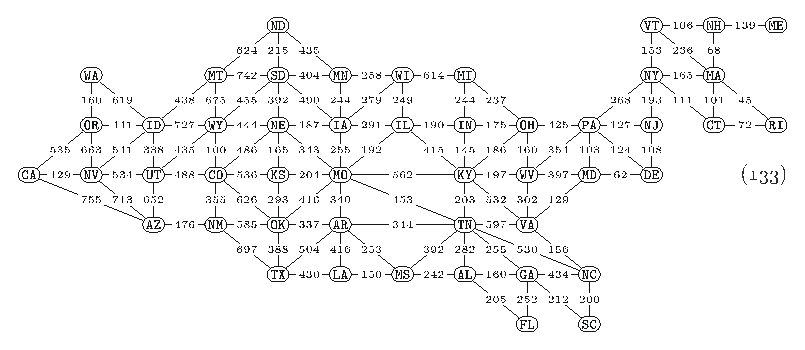
\includegraphics[width=0.7\linewidth]{fig/taocp_vol4fasc1b_p52_eq133.pdf}
  \end{minipage}
\end{figure}
%%%%%%%%%%%%%%%%%%%%%%%%%%%%%%%%%%%%%%%%%%%%%%%
\begin{itemize}
\item 1列目はコスト制約の閾値と最短距離からの倍率,2列目は解の総数,
  3列目以降は各符号化が解くのに要したCPU時間を示す.
\item \textsf{acyclicity}符号化が,より多くの問題を
  高速に解き,平均CPU時間ももっとも短かった.
\end{itemize}  
\end{frame}
%%%%%%%%%%%%%%%%%%%%%%%%%%%%%%%%%%%%%%%%%%%%%%%%%%%%%%%%%%%%%%%%%%%
\begin{frame}{まとめ}
    \begin{enumerate}
    \item \structure{ハミルトン閉路問題を解く3種類の ASP 符号化を考案.}
      \begin{itemize}
      \item ASP の高い表現力を生かし,ハミルトン閉路問題を簡潔に記述できることが確認できた.
      \end{itemize}
    \item \structure{既存のベンチマーク問題集を用いた評価実験.}
      \begin{itemize}
      \item ハミルトン閉路問題について,
        \textsf{directed}符号化の優位性が確認できた.
      \item 最短ハミルトン閉路問題については,
        \textsf{undirected}符号化の優位性を確認した.
      \item コスト制約付きハミルトン路問題については,
        \textsf{acyclicity}符号化の優位性を確認した.
      \end{itemize}
    \end{enumerate}
  \begin{alertblock}{今後の課題}
    \begin{itemize}
    \item 緩和問題と CEGAR (Counterexample Guided Abstraction Refinement) 
	  を用いた解法を応用した考案手法の高速化.
    \item 巡回セールスマン問題への拡張.
    \item 他手法との性能比較.
    \end{itemize}
  \end{alertblock}
\end{frame}
%%%%%%%%%%%%%%%%%%%%%%%%%%%%%%%%%%%%%%%%%%%%%%%%%%%%%%%%%%%%%%%%%%%
\begin{frame}[noframenumbering]{}
  補足
\end{frame}
%%%%%%%%%%%%%%%%%%%%%%%%%%%%%%%%%%%%%%%%%%%%%%%%%%%%%%%%%%%%%%%%%%%
% \begin{frame}[noframenumbering]{参考文献}
% \bibliographystyle{jplain} % 参考文献スタイル
% \bibliography{aisat,bachelor}    % 参考文献リスト
% \end{frame}
%%%%%%%%%%%%%%%%%%%%%%%%%%%%%%%%%%%%%%%%%%%%%%%%%%%%%%%%%%%%%%%%%%%

\end{document}

%%% Local Variables:
%%% mode: japanese-latex
%%% TeX-master: t
%%% End:
